%%%%%%%%%%%%%%%%%%%%%%%%%%%%%%%%%%%%%%%%%
% Jacobs Landscape Poster
% LaTeX Template
% Version 1.1 (14/06/14)
%
% Created by:
% Computational Physics and Biophysics Group, Jacobs University
% https://teamwork.jacobs-university.de:8443/confluence/display/CoPandBiG/LaTeX+Poster
% 
% Further modified by:
% Nathaniel Johnston (nathaniel@njohnston.ca)
%
% This template has been downloaded from:
% http://www.LaTeXTemplates.com
%
% License:
% CC BY-NC-SA 3.0 (http://creativecommons.org/licenses/by-nc-sa/3.0/)
%
%%%%%%%%%%%%%%%%%%%%%%%%%%%%%%%%%%%%%%%%%

%----------------------------------------------------------------------------------------
%	PACKAGES AND OTHER DOCUMENT CONFIGURATIONS
%----------------------------------------------------------------------------------------

\documentclass[final]{beamer}

\usepackage[scale=1.2]{beamerposter} % Use the beamerposter package for laying out the poster

\usetheme{confposter} % Use the confposter theme supplied with this template
\usepackage{tgbonum}
\setbeamercolor{block title}{fg=ngreen,bg=white} % Colors of the block titles
\setbeamercolor{block body}{fg=black,bg=white} % Colors of the body of blocks
\setbeamercolor{block alerted title}{fg=white,bg=dblue!70} % Colors of the highlighted block titles
\setbeamercolor{block alerted body}{fg=black,bg=dblue!10} % Colors of the body of highlighted blocks
% Many more colors are available for use in beamerthemeconfposter.sty

%-----------------------------------------------------------
% Define the column widths and overall poster size
% To set effective sepwid, onecolwid and twocolwid values, first choose how many columns you want and how much separation you want between columns
% In this template, the separation width chosen is 0.024 of the paper width and a 4-column layout
% onecolwid should therefore be (1-(# of columns+1)*sepwid)/# of columns e.g. (1-(4+1)*0.024)/4 = 0.22
% Set twocolwid to be (2*onecolwid)+sepwid = 0.464
% Set threecolwid to be (3*onecolwid)+2*sepwid = 0.708

\newlength{\sepwid}
\newlength{\onecolwid}
\newlength{\twocolwid}
\newlength{\threecolwid}
\setlength{\paperwidth}{48in} % A0 width: 46.8in
\setlength{\paperheight}{36in} % A0 height: 33.1in
\setlength{\sepwid}{0.01\paperwidth} % Separation width (white space) between columns
\setlength{\onecolwid}{0.23\paperwidth} % Width of one column
\setlength{\twocolwid}{0.464\paperwidth} % Width of two columns
\setlength{\threecolwid}{0.3\paperwidth} % Width of three columns
\setlength{\topmargin}{-0.9in} % Reduce the top margin size
%-----------------------------------------------------------

\usepackage{graphicx}  % Required for including images

% \usepackage{booktabs} % Top and bottom rules for tables

%----------------------------------------------------------------------------------------
%	TITLE SECTION 
%----------------------------------------------------------------------------------------

\title{ParkWizard: Street Parking Android App} % Poster title

\author{Siddharth Shah, Kunal Baweja, Dhruv Shekhawat, Anand Naik} % Author(s)

% \institute{\mbox{}} % Institution(s)

%----------------------------------------------------------------------------------------

\begin{document}

\addtobeamertemplate{block end}{}{\vspace*{1ex}} % White space under blocks
% \addtobeamertemplate{block alerted end}{}{\vspace*{2ex}} % White space under highlighted (alert) blocks

% \setlength{\belowcaptionskip}{2ex} % White space under figures
% \setlength\belowdisplayshortskip{2ex} % White space under equations

\begin{frame}[t] % The whole poster is enclosed in one beamer frame

\begin{columns}[t] % The whole poster consists of three major columns, the second of which is split into two columns twice - the [t] option aligns each column's content to the top

\begin{column}{\onecolwid} % The first column

%---------------
%	ABSTRACT
%--------------
\begin{alertblock}{Abstract}
\fontsize{34}{40} \selectfont A good day begins with a good parking. Finding a parking spot rather than ending up with a ticket is one of the daily struggles faced by millions of drivers worldwide, however the problem is not lack of parking, rather most of the times drivers are simply not aware of parking spots.\par
Various apps have been developed in the past but with an intention to provide paid garage parking. In this project, we introduce \textit{ParkWizard}, a user incentive based android app that crowdsources parking data to provide on-demand search facility for hassle free parking.
\end{alertblock}

%------------------
%	INTRODUCTION
%------------------

\begin{block}{Introduction}
\fontsize{34}{40} \selectfont \textit{ParkWizard} is an Android app that helps users find available street parking locations. It works on a score based system where users earn points by reporting parking locations and updating availability status. The users further spend their earned score back into the app to search for available parking spots when needed. This score-based system works well towards maintaining a smooth information flow between users(drivers) who want to find available parking spots and those(informers) who have information about them. At any point, a user can update as well as search for parking locations on the app.\par
\end{block}

\begin{block}{User Incentive \& Protocol Design}
\fontsize{34}{40} \selectfont \textit{Parkwizard} does not contain any parking location data of its own. It aims to incentivize users to provide the app with latest and most correct information about parking locations in their knowledge in return of earning reward points on the app. The scoring scheme is as follows:
\begin{itemize}
\fontsize{34}{40} \selectfont \item A user is rewarded 10 points for reporting a new parking location. However, a user is not allowed to report a parking within 50m of an already existing parking to avoid duplicates.

\fontsize{34}{40} \selectfont \item A user is rewarded 2 points for every update they provide about an existing parking spot. To limit misuse of the update feature, we limit a user to make a maximum of 5 updates per day. These updates can be made for parking spots within 100m of the user device location.

\fontsize{34}{40} \selectfont \item For updating false information such as suspiciously high number of parking spots or fake information, a user is penalized 2 points.

    % CONTINUED IN THIRD COLUMN
\end{itemize}

\end{block}

\end{column} % End of the first column

% Architecture
\begin{column}{\twocolwid} % The second column

\begin{block}{Algorithm}

% Algorithm Picture
\begin{figure}
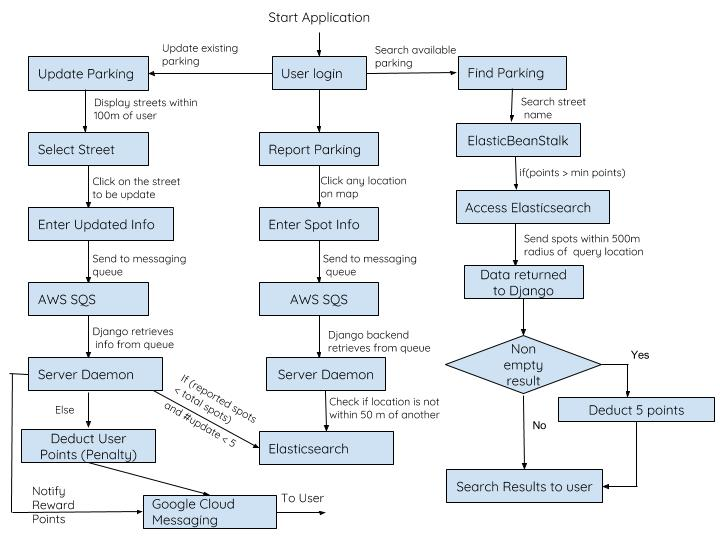
\includegraphics[width=54cm,height=40cm]{algorithm.jpg}
\caption{App State Transitions}
\end{figure}
\end{block}

% Vertical space hack
\vspace{1ex}

%Architecture Picture
\begin{figure}
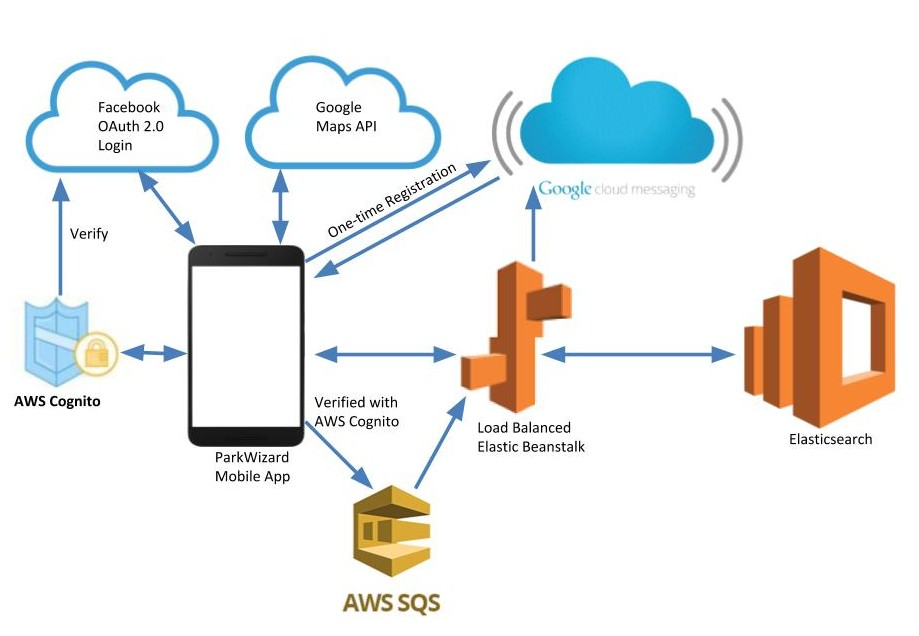
\includegraphics[width=47cm,height=29cm]{architecture.jpg}
\caption{Architecture}
\end{figure}

\end{column} % End of the second column

\begin{column}{\onecolwid} % The third column

\vspace{-2.2cm}
\begin{block}{}
\vspace{-1.3cm}
\begin{itemize}
\fontsize{34}{40} \selectfont \item A user has to spend 5 points to search for parking locations they wish to find near their destination. By default the parking locations are shown within a 500m radius of destination.

\fontsize{34}{40} \selectfont \item To encourage users to keep the parking location data most up to date, the app rewards them back 2 points if they choose to use a parking spot from the search results and navigates them to the location via Google Maps.
\end{itemize}
\end{block}

\vspace{-1.3cm}
\begin{block}{System Architecture \& Working}
\fontsize{34}{40} \selectfont Users sign up using Facebook OAuth 2.0 authentication. The app uses \textit{AWS Cognito service} to authenticate the user for accessing the underlying AWS services associated with \textit{ParkWizard}.\par

The server side business logic is implemented using Django 1.10.4, deployed on \textit{AWS ElasticBeanstalk} auto-scaling environment. This is backed by an auto-scaling deployment of \textit{AWS ElasticSearch} where the user and parking location data is indexed for fast real time searching.\par

\textit{Parkwizard} app uses \textit{Google Maps API} to display the geographical map as the primary user interface, where the user can see parking location search results, select parking locations to update available parking spots or report new parking locations from the menu option.\par

The user requests for searching parking locations and signing up require fast realtime processing and hence serviced directly by the servers deployed in \textit{AWS ElasticBeanstalk} auto-scaling environment. On the other hand, updates to parking locations and new locations need to be processed in order with some delay tolerance, for which we use the \textit{AWS SQS} service to queue up the requests. A continually running server daemon process, consumes the request messages from the SQS queue, updates the parking data on ElasticSearch and notifies users about score updates via push notifications sent through \textit{Google Cloud Messaging}.
\end{block}


%----------------
%	CONCLUSION
%----------------

\setbeamercolor{block alerted title}{fg=black,bg=norange} % Change the alert block title colors
\setbeamercolor{block alerted body}{fg=black,bg=white} % Change the alert block body colors

\begin{alertblock}{Conclusion}
\fontsize{34}{40} \selectfont \textit{ParkWizard's} mission is to solve the tedious problem of daily parking as the cities grow more and more complex. The user incentive based approach for crowd sourcing latest information about parking location also ensures cheap, reliable and efficient data collection of parking locations which in turn results in most relevant search results and user activity.
\end{alertblock}

\end{column} % End of the third column

\end{columns} % End of all the columns in the poster

\end{frame} % End of the enclosing frame

\end{document}
